\documentclass[UTF8,zihao=-4,fontset=windows]{ctexart}

\usepackage[a4paper,top=2.2cm,bottom=2.2cm,left=2.45cm,right=2.45cm]{geometry}
\usepackage{graphicx}
\usepackage{booktabs}
\usepackage{tabularx}
\usepackage{array}
\usepackage{enumitem}
\usepackage{amsmath}
\usepackage{amssymb}
\usepackage{xcolor}
\usepackage{xurl}
\usepackage{hyperref}
\usepackage{fancyhdr}
\usepackage{caption}
\usepackage{float}
\usepackage{titlesec}
\usepackage[most]{tcolorbox}
\usepackage{tikz}
\usepackage{pgfplots}
\usetikzlibrary{arrows.meta,positioning,calc,fit,shapes.geometric}
\pgfplotsset{compat=1.18}

\definecolor{mpddblue}{HTML}{1F4E79}
\definecolor{mpddcyan}{HTML}{168C8C}
\definecolor{mpddorange}{HTML}{D97904}
\definecolor{mpddpurple}{HTML}{6551C5}
\definecolor{mpddgray}{HTML}{4D5663}
\definecolor{mpddlight}{HTML}{F3F7FB}
\definecolor{mpddline}{HTML}{D8E3EF}
\definecolor{mpdddark}{HTML}{102033}

\hypersetup{
  unicode=true,
  colorlinks=true,
  linkcolor=mpddblue,
  urlcolor=mpddblue,
  citecolor=mpddblue,
  pdftitle={面向PHQ-9预测的多模态抑郁检测期末大作业文档},
  pdfauthor={张子路 郭子逸 龚正硕 丁一鸣 蒋一鸣 谈亮}
}

\graphicspath{{assets/ppt_media/}}
\pagestyle{fancy}
\fancyhf{}
\lhead{\small 语音信息处理期末大作业}
\rhead{\small MPDD-AVG Young 多模态抑郁检测}
\cfoot{\thepage}
\setlength{\headheight}{15pt}
\linespread{1.08}
\setlength{\parindent}{2em}
\setlength{\parskip}{0.16em}
\setlist[itemize]{leftmargin=2em,itemsep=0.16em,topsep=0.16em}
\setlist[enumerate]{leftmargin=2em,itemsep=0.16em,topsep=0.16em}
\renewcommand{\arraystretch}{1.18}
\captionsetup{font=small,labelfont=bf}
\emergencystretch=2em

\titleformat{\section}
  {\Large\bfseries\color{mpdddark}}
  {\thesection}{0.9em}{}
\titleformat{\subsection}
  {\large\bfseries\color{mpddblue}}
  {\thesubsection}{0.8em}{}
\titlespacing*{\section}{0pt}{1.6em}{0.8em}
\titlespacing*{\subsection}{0pt}{1.0em}{0.45em}

\newcommand{\code}[1]{\texttt{#1}}
\newcommand{\fpath}[1]{\path{#1}}
\newcommand{\phq}{PHQ-9}
\newcommand{\ccc}{CCC}
\newcommand{\score}{Score}
\newcommand{\tightcaption}[1]{\caption{#1}\vspace{-0.4em}}

\newtcolorbox{takeawaybox}{
  enhanced,
  breakable,
  colback=mpddlight,
  colframe=mpddblue,
  boxrule=0.7pt,
  arc=2mm,
  left=1.0em,
  right=1.0em,
  top=0.75em,
  bottom=0.75em
}

\newtcolorbox{methodbox}[1]{
  enhanced,
  breakable,
  colback=white,
  colframe=mpddline,
  borderline west={2.5pt}{0pt}{mpddblue},
  boxrule=0.45pt,
  arc=1.5mm,
  title={#1},
  coltitle=mpdddark,
  fonttitle=\bfseries,
  colbacktitle=mpddlight,
  left=0.9em,
  right=0.9em,
  top=0.55em,
  bottom=0.55em
}

\begin{document}

\begin{titlepage}
  \centering
  \vspace*{0.35cm}
  {\Large 语音信息处理期末大作业\par}
  \vspace{0.75cm}
  {\zihao{1}\bfseries\color{mpdddark} 面向 \phq 预测的多模态抑郁检测\par}
  \vspace{0.28cm}
  {\zihao{3}\bfseries\color{mpddblue} 行为动态特征、稳健融合与语音探索\par}
  \vspace{0.7cm}
  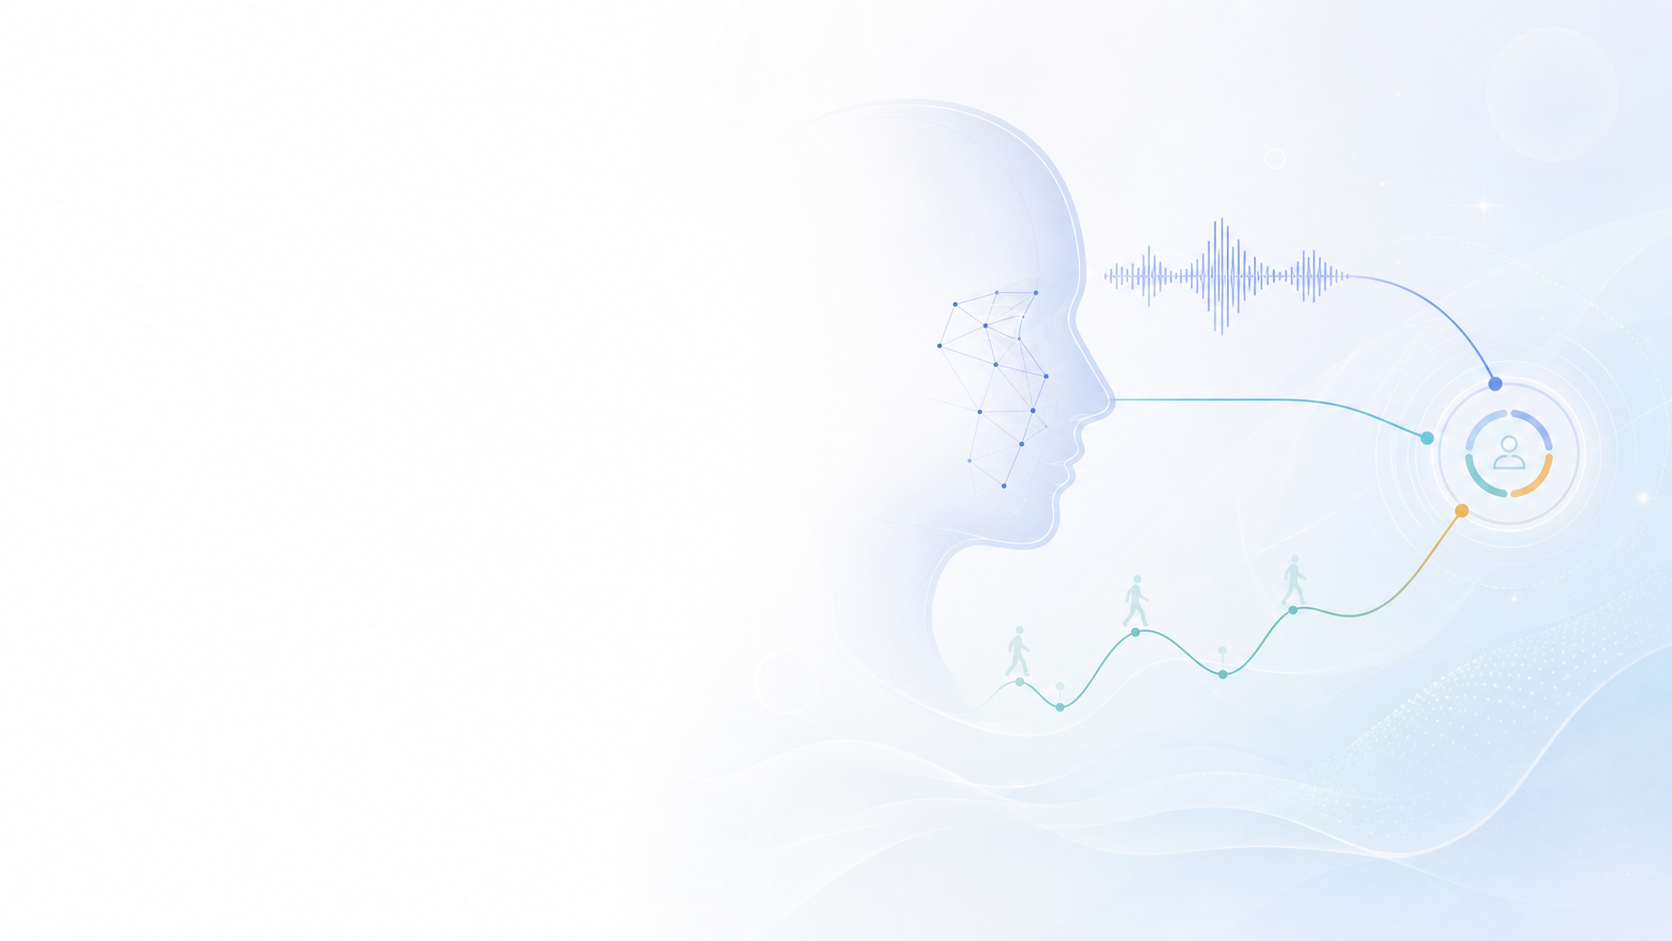
\includegraphics[width=0.86\linewidth]{image1.png}
  \vspace{0.62cm}

  \begin{tcolorbox}[enhanced,colback=white,colframe=mpddline,boxrule=0.6pt,arc=2mm,width=0.86\linewidth]
  \centering
  \begin{tabularx}{0.95\linewidth}{>{\bfseries}lX}
    小组成员 & 张子路、郭子逸、龚正硕、丁一鸣、蒋一鸣、谈亮 \\
    代码仓库 & \url{https://github.com/ZZL-2005/mpdd-bupt666-coderepo} \\
  \end{tabularx}
  \end{tcolorbox}
\end{titlepage}

\pagenumbering{Roman}
\begin{abstract}
本项目围绕 MPDD-AVG 2026 Young Track 的多模态抑郁检测任务展开。任务要求根据青年受试者的访谈音视频、IMU 步态和人格描述信息，同时输出 \phq 连续分数、二分类标签和三分类标签。数据规模是项目方法选择的核心约束：训练集只有 88 人，测试集 22 人，而音频、视频和 IMU 都是变长时序；若直接使用高维深度表征或端到端网络，模型很容易学习到个体差异、录音条件和偶然表达，而不是真正稳定的抑郁线索。

我们的技术路线不是堆叠所有模态，而是在竞赛反馈和本地验证中逐步筛选有效信号。首先以 IMU 前三维加速度和 Big Five 人格构成有序回归主干；随后发现 OpenFace gaze/AU 动态能补充主干无法覆盖的表情运动信息，并将其拆分为速度、后段状态、疲劳轨迹和频谱节律四路 ranker；最后通过 \ccc 分布校准解决回归输出收缩问题，通过双模态一致性规则处理分类边界。作为语音信息处理课程项目，我们还系统探索了 openSMILE、MFCC、wav2vec2、GRU + attention、ASR + \phq 语义证据以及 e2speech 发音迟缓特征。实验表明，语音线具有解释价值，但在 88 人训练规模下没有形成稳定 hidden-test 增益，因此最终作为负面结论和方法贡献保留。最终提交综合分约 0.87，其中连续回归 \ccc 约为 0.8772。

\noindent\textbf{关键词：} 抑郁检测；语音信号处理；OpenFace；IMU；\phq；一致性相关系数；小样本学习
\end{abstract}

\tableofcontents
\clearpage
\pagenumbering{arabic}

\section{选题背景}

\subsection{MPDD-AVG 2026 挑战赛介绍}

本项目来源于 MPDD-AVG Challenge 2026。该挑战赛是 ACM Multimedia 2026 Grand Challenge，主题为 Multimodal Personality-Aware Depression Detection via Audio-Visual Interview and Gait Analysis，目标是利用访谈和步态监测中的多模态行为信号估计受试者抑郁严重程度。\footnote{MPDD-AVG Challenge 2026 官网：\href{https://hacilab.github.io/MPDD-AVG-2026.github.io/challenge.html}{challenge page}.}

这个任务与传统只使用语音、文本或单一视频特征的抑郁识别不同。它同时包含访谈音频、面部/视频行为、IMU 步态和人格特质，因此模型需要判断多种行为信号是否共同指向抑郁状态。对语音信息处理课程而言，它覆盖了声学表征、语音识别、说话状态分析和多模态情感计算等方向；对机器学习而言，它又是典型的小样本、多模态、指标不一致问题。

挑战赛按年龄组划分为 MPDD-Young 和 MPDD-Elderly。本项目选择 Young 数据作为实验对象，一方面因为青年群体贴近大学生心理健康场景，另一方面因为该子集样本少、模态丰富，能很好地体现“哪些模态值得信任，哪些模态只是在小样本下制造过拟合”这一核心问题。

\subsection{数据集结构说明}

MPDD-Young 共包含 110 名青年受试者。本地数据核对显示，其中 88 人有训练标签，22 人作为测试集；训练集提供 \phq 连续分数、二分类标签和三分类标签，测试集只提供待预测样本的多模态数据。人格描述与 Big Five 提取结果覆盖全部 110 人。

\begin{figure}[H]
  \centering
  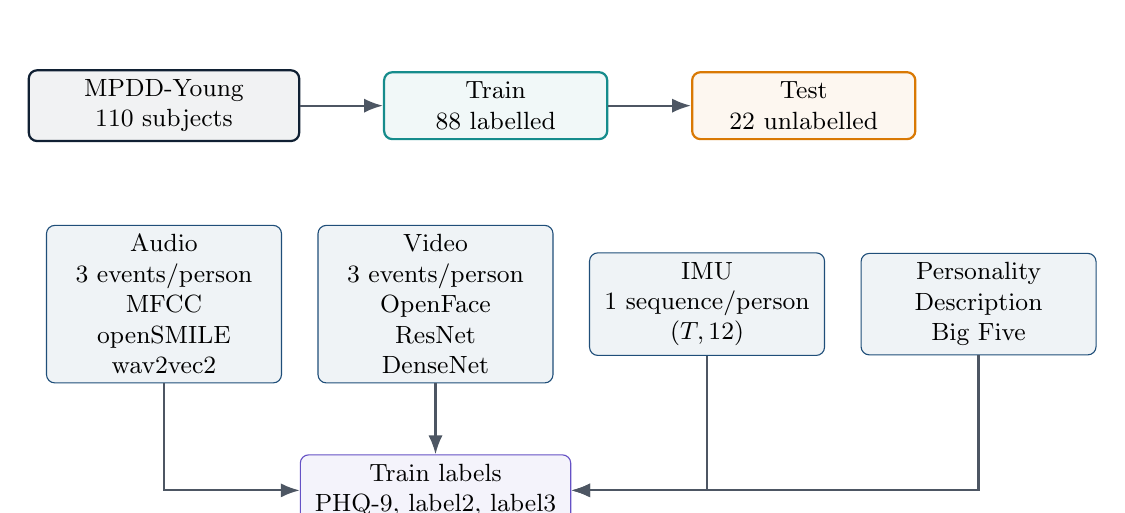
\begin{tikzpicture}[
    font=\small,
    node distance=0.55cm,
    box/.style={draw=#1,fill=#1!6,rounded corners=3pt,minimum height=0.85cm,align=center,text width=2.6cm,thick},
    data/.style={draw=mpddblue,fill=mpddblue!7,rounded corners=3pt,minimum height=0.82cm,align=center,text width=2.75cm},
    arr/.style={-{Latex[length=2.4mm]},thick,draw=mpddgray}
  ]
    \node[box=mpdddark,text width=3.2cm] (all) {MPDD-Young\\110 subjects};
    \node[box=mpddcyan,right=1.05cm of all] (train) {Train\\88 labelled};
    \node[box=mpddorange,right=1.05cm of train] (test) {Test\\22 unlabelled};
    \draw[arr] (all) -- (train);
    \draw[arr] (train) -- (test);

    \node[data,below=1.05cm of all] (audio) {Audio\\3 events/person\\MFCC\\openSMILE\\wav2vec2};
    \node[data,right=0.45cm of audio] (video) {Video\\3 events/person\\OpenFace\\ResNet\\DenseNet};
    \node[data,right=0.45cm of video] (imu) {IMU\\1 sequence/person\\$(T,12)$};
    \node[data,right=0.45cm of imu] (pers) {Personality\\Description\\Big Five};
    \node[draw=mpddpurple,fill=mpddpurple!7,rounded corners=3pt,minimum height=0.85cm,align=center,text width=3.2cm,below=0.9cm of video] (labels) {Train labels\\\phq, label2, label3};
    \draw[arr] (audio.south) |- (labels.west);
    \draw[arr] (video.south) -- (labels.north);
    \draw[arr] (imu.south) |- (labels.east);
    \draw[arr] (pers.south) |- (labels.east);
  \end{tikzpicture}
  \tightcaption{MPDD-Young 数据结构与本项目使用的信息}
  \label{fig:dataset-structure}
\end{figure}

\begin{table}[H]
  \centering
  \caption{本地核对后的主要文件与规模}
  \begin{tabularx}{\linewidth}{l c c X}
    \toprule
    数据项 & 训练集 & 测试集 & 说明 \\
    \midrule
    受试者人数 & 88 & 22 & 训练标签位于 \code{split\_labels\_train.csv}；测试标签不公开。 \\
    原始音频/视频 & 264/264 & 66/66 & 每人 3 段 event，文件名为 \code{event\_1} 至 \code{event\_3}。 \\
    音频特征 & 264 files & 66 files & \code{mfcc64} 64 维、\code{opensmile} 65 维、\code{wav2vec2} 1024 维。 \\
    视频特征 & 264 files & 66 files & \code{openface} 710 维、\code{resnet}/\code{densenet} 1000 维。 \\
    IMU 特征 & 88 files & 22 files & 每人一个变长序列，形状为 $(T,12)$，最终主干只用前三维加速度。 \\
    人格信息 & \multicolumn{2}{c}{110 rows} & \code{descriptions.csv} 与 Big Five 提取表覆盖训练和测试全体。 \\
    \bottomrule
  \end{tabularx}
\end{table}

\subsection{标签分布与建模约束}

训练标签分布直接影响模型设计。训练集 \phq 均值为 4.818，标准差为 3.486，范围为 0--17；实际出现的分值只有 0,1,2,3,4,5,6,7,8,9,10,11,16,17。这里的“缺失”不是 CSV 中存在空值，而是训练集中没有 12--15 和 18--27 这些分段的样本。

\begin{figure}[H]
  \centering
  \begin{tikzpicture}
    \begin{axis}[
      width=0.92\linewidth,
      height=5.2cm,
      ybar,
      bar width=10pt,
      ymin=0,
      ymax=16,
      ylabel={人数},
      xlabel={训练集 \phq 分数},
      symbolic x coords={0,1,2,3,4,5,6,7,8,9,10,11,16,17},
      xtick=data,
      axis lines*=left,
      ymajorgrids=true,
      grid style={mpddline},
      tick label style={font=\small},
      label style={font=\small},
      nodes near coords,
      nodes near coords style={font=\scriptsize},
      every axis plot/.append style={fill=mpddblue!65,draw=mpddblue}
    ]
      \addplot coordinates {(0,7) (1,9) (2,9) (3,10) (4,10) (5,8) (6,15) (7,4) (8,2) (9,4) (10,4) (11,4) (16,1) (17,1)};
    \end{axis}
  \end{tikzpicture}
  \tightcaption{训练集 \phq 取值分布：离散、右偏且高分样本稀少}
  \label{fig:phq-dist}
\end{figure}

二分类 label2 为 45/43，基本平衡；三分类 label3 为 45/33/10，其中重度类只有 10 人。这意味着三分类 Kappa 对少数几个样本极其敏感，也解释了为什么后期不能只优化 \phq 排序，还必须单独处理分类边界。

\begin{takeawaybox}
\textbf{数据约束带来的方法原则：} 训练样本只有 88 人，而 OpenFace、wav2vec2、视频嵌入等表征都是高维变长序列。最终有效方法必须控制维度、控制参数量，并把每一个新增特征都解释为具体行为线索。项目真正的难点不是训练一个更大的网络，而是在小样本和多指标约束下判断哪些信号可以泛化。
\end{takeawaybox}

\section{实验目标}

\subsection{Young 子赛道情况}

MPDD-Young 按允许使用的模态组合设置多个子赛道。三个 Young 子赛道的预测目标一致，都需要提交 \phq 连续预测、二分类预测和三分类预测；区别在于可使用的数据范围不同。

\begin{table}[H]
  \centering
  \caption{MPDD-Young 子赛道与允许使用的数据}
  \begin{tabularx}{\linewidth}{lX X}
    \toprule
    子赛道 & 允许使用的数据 & 任务侧重点 \\
    \midrule
    Young A-V+P & 访谈音频、视频/面部行为、Big Five 人格。 & 从说话状态、面部行为和人格差异中识别抑郁线索。 \\
    Young A-V-G+P & 音频、视频/面部、IMU 步态、Big Five 人格。 & 完整多模态融合，综合访谈行为与步态行为。 \\
    Young G+P & IMU 步态、Big Five 人格。 & 考察步态心理运动迟缓与人格因素的预测能力。 \\
    \bottomrule
  \end{tabularx}
\end{table}

\subsection{本项目目标}

本项目的目标不是只提交一次结果，而是完成一个围绕 MPDD-Young 的综合实验项目：
\begin{enumerate}
  \item 构建可复现的 \phq 回归、二分类和三分类提交流程，理解 \score、F1、\ccc、Kappa 之间的关系。
  \item 系统比较 IMU、人格、面部动态和语音相关信号的有效性，说明哪些模态进入最终模型，哪些模态作为负面结论保留。
  \item 结合课程方向，重点分析语音声学、深度语音表征、ASR 语义证据在小样本抑郁检测中的作用和边界。
  \item 形成不包含数据和模型权重的代码交付包，明确复现入口、依赖、缓存文件和提交格式。
\end{enumerate}

从最终方案看，我们以 G+P 稳定主干为锚点，引入 OpenFace 面部动态形成 Young A-V-G+P 允许范围内的多模态融合方案。这里的 A-V-G+P 表示该子赛道允许使用音频、视频、步态和人格数据；我们的最终提交实际使用其中的 IMU、Big Five 和 OpenFace 视频特征，没有把语音特征纳入主融合。语音线没有进入主提交，但作为课程相关探索和失败分析写入报告。这一取舍来自实验结果，而不是忽略语音模态。

\section{方法流程与探索过程}

本章按实际探索顺序组织。每个小节都回答四个问题：为什么尝试这条路线、具体怎么实现、实验反馈是什么、最后如何取舍。图 \ref{fig:method-pipeline} 给出最终系统与语音探索线之间的关系。

\begin{figure}[H]
  \centering
  \resizebox{\linewidth}{!}{
  \begin{tikzpicture}[
    font=\small,
    box/.style={draw=mpddblue,fill=mpddblue!6,rounded corners=3pt,minimum height=1.05cm,text width=2.5cm,align=center,thick},
    face/.style={draw=mpddcyan,fill=mpddcyan!7,rounded corners=3pt,minimum height=1.05cm,text width=2.7cm,align=center,thick},
    warn/.style={draw=mpddorange,fill=mpddorange!7,rounded corners=3pt,minimum height=1.05cm,text width=2.9cm,align=center,thick},
    outbox/.style={draw=mpddpurple,fill=mpddpurple!7,rounded corners=3pt,minimum height=1.05cm,text width=2.75cm,align=center,thick},
    arr/.style={-{Latex[length=2.5mm]},thick,draw=mpddgray}
  ]
    \node[box] (imu) {IMU accel3\\+ Big Five};
    \node[box,right=0.65cm of imu] (orig) {OrdinalRidge\\ORIG 主干};
    \node[face,above=1.05cm of orig] (of) {OpenFace 43 cols\\gaze/AU};
    \node[face,right=0.65cm of of] (ranker) {4 face rankers\\auvel/e3only\\fatigue/auspec};
    \node[warn,below=1.05cm of ranker] (speech) {Speech exploration\\openSMILE\\wav2vec2\\ASR/e2speech};
    \node[outbox,right=0.7cm of ranker] (blend) {weighted blend\\ORIG + face};
    \node[outbox,right=0.65cm of blend] (calib) {\ccc calibration\\moment matching};
    \node[outbox,right=0.65cm of calib] (cls) {classification head\\AND rule};
    \node[box,right=0.65cm of cls] (sub) {submission.zip\\binary/ternary};
    \draw[arr] (imu) -- (orig);
    \draw[arr] (of) -- (ranker);
    \draw[arr] (orig) -- (blend);
    \draw[arr] (ranker) -- (blend);
    \draw[arr] (blend) -- (calib);
    \draw[arr] (calib) -- (cls);
    \draw[arr] (cls) -- (sub);
    \draw[arr,dashed,draw=mpddorange] (speech) -- node[right,font=\scriptsize,align=center]{负面验证\\不进最终融合} (ranker);
  \end{tikzpicture}}
  \tightcaption{最终方法管线：稳定主干、面部动态补充、指标校准与分类收口}
  \label{fig:method-pipeline}
\end{figure}

\subsection{探索一：G+P 主干复现}

\begin{methodbox}{动机}
项目的第一步不是直接融合所有模态，而是先建立一个稳定锚点。IMU 步态和人格特质维度低、解释清楚，适合作为 Young G+P 主干；如果后续模态不能超过或补充这个主干，就不应进入最终系统。
\end{methodbox}

实现上，我们只取 IMU 前三维加速度 $a_x,a_y,a_z$，提取频带能量比例、自相关周期、步伐峰间隔、三轴相关性、合加速度幅值统计等约 33 维步态特征；再从人格描述中解析 Big Five 五项分数，拼成约 38 维输入。模型使用 \code{StandardScaler + OrdinalRidge}。之所以把 \phq 当作有序标签，是因为训练集中 \phq 是离散且不连续的，直接连续回归容易在 12--15 等无样本区间外推。

该主干独立得分约 0.67。它的价值不只在分数，而在于后续所有特征都可以围绕它判断：是提供了互补信息，还是只是重复了 IMU/人格已经表达的内容。

\subsection{探索二：早期融合筛选}

复现 ORIG 后，我们尝试过 ORIG 与单独 IMU 项、早期音频统计、高维 embedding、初步 OpenFace 特征的线性融合。这个阶段的任务是筛选方向，而不是追求最终最优。

实验反馈很快暴露出几个问题。单独再加入 IMU 项大多与 ORIG 冗余，因为 ORIG 已经吸收了最稳定的步态信息；早期音频特征在本地验证上偶尔有提升，但榜单反馈不稳定；高维 embedding 容易把样本偶然性带入模型。相对而言，OpenFace 面部动态开始显示出更稳定的互补性。由此我们形成了后续筛选准则：新特征必须与主干适度互补、具有行为学解释，并且维度和模型容量要匹配 88 人样本量。

\subsection{探索三：OpenFace 面部 AU 突破}

面部方向的临床动机是心理运动迟缓。抑郁状态可能表现为表情幅度减小、变化速度下降、注视和动作单元激活模式改变。OpenFace 原始每帧 710 维，如果直接使用全量特征，维度远高于样本量；因此我们去掉第 0 列帧号后，只保留 gaze 0--7、AU intensity 674--690、AU presence 691--708，共 43 个关键列。

\begin{table}[H]
  \centering
  \caption{OpenFace 关键列选择}
  \begin{tabularx}{0.88\linewidth}{l c X}
    \toprule
    组别 & 维度 & 作用 \\
    \midrule
    gaze & 8 & 注视方向和眼部运动线索。 \\
    AU intensity & 17 & 面部动作单元的连续强度。 \\
    AU presence & 18 & 面部动作单元是否出现。 \\
    \midrule
    合计 & 43 & 保留与表情运动学最直接相关的维度。 \\
    \bottomrule
  \end{tabularx}
\end{table}

引入这 43 维 OpenFace 特征后，Score 从约 0.68 提升到约 0.706，\ccc 从约 0.55 提升到约 0.62。这是项目中的第一次实质突破：面部动态捕捉的是步态和人格没有覆盖的行为层面，因此比简单堆叠更多 IMU 或 embedding 更有效。

\subsection{探索四：四路面部 ranker}

确认 OpenFace 有效后，我们没有把所有面部统计粗暴拼接，而是把“面部运动迟缓”拆成四个互补视角：

\begin{table}[H]
  \centering
  \caption{四路面部动态 ranker}
  \begin{tabularx}{\linewidth}{l c X X}
    \toprule
    ranker & 维度 & 构造方式 & 行为含义 \\
    \midrule
    auvel & 387 & 三段 event 分别取 mean/std/mean($|\Delta|$)，再拼接。 & 表情活跃度和变化速度。 \\
    e3only & 129 & 只取 event 3 的 mean/std/mean($|\Delta|$)。 & 任务后段状态，可能暴露疲劳和注意力下降。 \\
    fatigue & 129 & 计算 $\mu_2-\mu_1,\mu_3-\mu_2,\mu_3-\mu_1$。 & 随任务推进的表情均值漂移。 \\
    auspec & 645 & 对 AU 时序做 FFT，提取三频带能量、谱熵和主频。 & 表情节律是否单调、低频化。 \\
    \bottomrule
  \end{tabularx}
\end{table}

这四路 ranker 都来自同一组 43 列 OpenFace，但关注点不同。auvel 看速度，e3only 看后段状态，fatigue 看跨事件变化，auspec 看频谱节律。这样的拆法比“全量拼特征”更可解释，也更符合小样本下的维度控制要求。

\subsection{探索五：\ccc-loss MLP 与多 seed 集成}

面部特征进入模型时，我们使用统一的浅层 MLP 配方：输入维度 $d$，两层隐藏层 96 和 48，激活函数为 GELU，dropout 为 0.3；优化器为 AdamW，学习率 $10^{-3}$，weight decay $10^{-3}$，训练 400 epoch。损失函数以 \ccc loss 为主，并加入轻量 MSE 正则：
\[
\mathcal{L}=(1-\mathrm{CCC})+0.1\cdot\mathrm{MSE}.
\]

为了降低 88 人小样本下的训练随机性，每一路 ranker 训练 50 个 seed，并在训练中使用 mixup 生成虚拟样本。最终每一路预测取 50 个 seed 的平均。换句话说，我们没有依赖某一次深度训练的幸运结果，而是用浅层模型和多 seed 集成获得更稳定的排序信号。

\subsection{探索六：\ccc 分布校准}

当四路面部 ranker 已经能给出较好的排序后，新的瓶颈变成 \ccc。它不只看相关性，还同时惩罚均值偏移和方差失配：
\[
\mathrm{CCC}(y,\hat y)=\frac{2\,\mathrm{Cov}(y,\hat y)}
{\mathrm{Var}(y)+\mathrm{Var}(\hat y)+(\bar y-\bar{\hat y})^2}.
\]

小样本回归常见的问题是预测值向均值收缩：排序可能还可以，但预测分布过窄，方差小于真实标签分布，从而压低 \ccc。我们的做法是对融合后的 \phq 预测做 moment matching，把预测均值和标准差对齐到训练集 \phq 的统计量：
\[
\hat y_{\mathrm{cal}}=(\hat y-\mu_{\hat y})\frac{\sigma_{\mathrm{target}}}{\sigma_{\hat y}}+\mu_{\mathrm{target}}.
\]

这一步基本不改变样本排序，却显著修正了 \ccc 分母中的方差项。实验上，\ccc 从约 0.65 提升到 0.8772，Score 从约 0.72 提升到约 0.79。它说明本任务后期的主要收益不是继续堆模态，而是理解指标并修正输出分布。

\subsection{探索七：独立分类头}

最初我们直接用 \phq 阈值导出二分类和三分类，但当 \ccc 提升到 0.8772 后，F1 与 Kappa 仍长期停滞。这说明“连续严重程度排序好”和“分类边界判断好”不是同一个问题。

最终分类头采用双模态一致性规则。二分类阳性要求融合 \phq 预测超过阈值 $t_1=4.25$，同时 ORIG 主干也给出不低的步态/人格证据；三分类在此基础上使用 $t_2=11$ 判断重度。可以概括为：
\[
\text{positive} = [\mathrm{PHQ}_{\mathrm{blend}}\geq 4.25]\ \land\ [\mathrm{ORIG}\geq 4].
\]

这一规则的意义是降低单一模态误报。若面部模型认为某个样本有迟缓迹象，但 IMU/人格主干强烈反对，就不直接判阳性。分类头阶段把综合分提升到约 0.8347，其中 F1 约 0.8255，Kappa 约 0.8012。

\subsection{探索八：语音声学与嵌入特征}

作为语音信息处理课程项目，语音线是我们必须认真处理的部分。数据提供了 MFCC64、openSMILE 65 维低层声学描述子、wav2vec2 1024 维自监督嵌入，同时也有可用于 ASR 的原始音频。我们尝试从音高、能量、嗓音质量、语速、韵律和深层声学表征中寻找抑郁线索。

实验结果并不稳定。部分 openSMILE 与 IMU 的早期融合在本地验证上出现过提升，但 hidden test 没有兑现；wav2vec2 维度高、帧数长，在 88 人样本下尤其容易过拟合。我们的判断是，语音声学特征同时受口音、说话习惯、麦克风条件、访谈内容密度影响，这些因素不一定和抑郁状态稳定相关。

\subsection{探索九：语音深度序列模型}

为了验证深度时序模型是否能直接捕捉访谈中的时间依赖，我们在 openSMILE 和 wav2vec2 时序上尝试 GRU + attention pooling。理论上，这类模型可以学习说话过程中的动态变化；但在当前样本规模下，模型容量明显超过监督信号规模。

\begin{table}[H]
  \centering
  \caption{语音深度序列模型负面结果}
  \begin{tabular}{lcc}
    \toprule
    输入/模型 & binary F1 & ternary Kappa \\
    \midrule
    手工特征基线 & 0.7972 & 0.7048 \\
    openSMILE + GRU & 0.5856 & 0.0421 \\
    wav2vec2 + GRU & 0.5227 & 0.1758 \\
    \bottomrule
  \end{tabular}
\end{table}

结果显示，深度语音序列模型没有超过基线，反而明显下降。这一负面结果很重要：在小样本抑郁检测里，深度模型的形式复杂并不自动转化为泛化能力。

\subsection{探索十：e2speech 发音迟缓特征}

e2speech 是语音线中最有设计动机的一次尝试。前面面部 auvel 证明 mean($|\Delta|$) 可以刻画表情运动速度，因此我们把同样思想迁移到语音：如果抑郁相关的心理运动迟缓会表现在发音上，那么 openSMILE 低层声学描述子的帧间变化幅度可能也会下降。

实现上，我们选取 event 2 的 openSMILE 65 维时序，提取 mean、std 和 mean($|\Delta|$) 三类统计，共 195 维；模型沿用浅层 \ccc-loss MLP 与多 seed 集成。这个设计的解释性较强：它不是盲目使用语音特征，而是把面部运动迟缓迁移为发音迟缓。然而 hidden test 没有稳定增益，因此最终没有进入主融合。

\subsection{探索十一：ASR + \phq 语义证据}

另一条语音线关注“说了什么”。我们使用 DashScope qwen3-asr-flash 对 event 1 访谈语音转写，再围绕 \phq 九个条目构造 direct、weak、protective 三类关键词证据，覆盖睡眠、疲劳、兴趣、情绪、自我评价、活动意愿等域。证据被整理为 item prior，再汇总为 \phq 总分和二/三分类。

这条线的优点是可解释：可以说明预测来自哪些症状语义证据。其独立提交结果为 Score 0.457751、F1 0.583333、\ccc 0.508394、Kappa 0.281525，弱于 IMU 主干。原因主要在于转写错误和关键词规则会放大偶然表达，“提到某个词”并不等价于稳定的 \phq 证据。因此 ASR 线被保留为课程相关探索和错误分析材料，而不进入最终模型。

\section{实验结果}

\subsection{最终提交方案与赛道定位}

最终提交名为 \code{young\_final\_t4p25\_t2p11}。从赛道定位看，由于方案使用了 OpenFace 视频特征、IMU/Gait 与 Personality，属于 Young A-V-G+P 子赛道允许的数据范围；但从实际建模看，它并不是把所有官方模态无差别堆叠的全模态模型。它以 IMU 步态与 Big Five 人格作为稳定主干，引入 OpenFace 面部动态特征进行融合；语音模态作为系统探索与负面结果保留，没有进入最终提交。

连续预测由五路分数组成：
\[
\mathrm{raw}=0.40\,\mathrm{ORIG}+0.30\,\mathrm{auvel}+0.20\,\mathrm{e3only}+0.10\,\mathrm{fatigue}+0.05\,\mathrm{auspec}.
\]
随后对 raw 做 \phq 分布校准，再用 $t_1=4.25,t_2=11$ 和 ORIG 双确认规则生成二分类与三分类提交。

\subsection{阶段性结果}

\begin{figure}[H]
  \centering
  \begin{tikzpicture}
    \begin{axis}[
      width=0.92\linewidth,
      height=5.4cm,
      ymin=0.62,
      ymax=0.89,
      ylabel={榜单导向综合分},
      symbolic x coords={ORIG,Face AU,Rankers,Calibration,Classifier,Final},
      xtick=data,
      ymajorgrids=true,
      grid style={mpddline},
      axis lines*=left,
      tick label style={font=\small},
      x tick label style={rotate=18,anchor=east},
      label style={font=\small},
      mark=*,
      nodes near coords,
      nodes near coords style={font=\scriptsize,anchor=south},
      every axis plot/.append style={very thick,draw=mpddblue,fill=mpddblue}
    ]
      \addplot coordinates {(ORIG,0.670) (Face AU,0.706) (Rankers,0.718) (Calibration,0.793) (Classifier,0.834) (Final,0.870)};
    \end{axis}
  \end{tikzpicture}
  \tightcaption{方法演进里程碑：提升来自阶段性问题解决，而非单纯换大模型}
  \label{fig:milestone}
\end{figure}

\begin{table}[H]
  \centering
  \caption{关键版本结果概览}
  \begin{tabularx}{0.92\linewidth}{l c X}
    \toprule
    版本/阶段 & 指标 & 说明 \\
    \midrule
    ORIG 主干 & Score $\approx 0.67$ & IMU 三轴加速度 + Big Five，有序回归。 \\
    OpenFace AU & Score $\approx 0.706$ & 面部动态提供首次稳定增益。 \\
    四路 ranker & Score $\approx 0.718$ & 速度、后段状态、疲劳、频谱四视角。 \\
    \ccc 校准 & Score $\approx 0.793$，\ccc=0.8772 & 分布校准修正回归输出收缩。 \\
    分类头 & Score $\approx 0.8347$ & 双模态一致性规则提升 F1/Kappa。 \\
    最终提交 & Score $\approx 0.87$ & \code{young\_final\_t4p25\_t2p11}。 \\
    ASR V4 & Score=0.457751 & 可解释语义线，未进入最终融合。 \\
    \bottomrule
  \end{tabularx}
\end{table}

现有材料中可可靠核对的最终精确值包括综合分约 0.87 与 \ccc=0.8772；最终 F1/Kappa 的完整小数没有在交付材料中保留，因此本文不伪造精确值。报告中所有精确小数均来自可核对的技术文档、提交记录或 ASR 结果文件。

\section{问题分析与认识}

\subsection{小样本决定了方法上限}

MPDD-Young 的训练样本只有 88 人，而每个模态都可以产生大量特征。若把 wav2vec2、ResNet、DenseNet、OpenFace 全量拼接后训练复杂模型，参数量与特征维度会远超样本规模。实验中的 BiLSTM、GRU、LightGBM、Random Forest 等尝试都说明：更复杂的模型不一定更强，反而更容易记住训练分布的偶然性。

\subsection{本地验证不能替代隐藏测试反馈}

小样本还带来一个直接问题：本地 LOO/CV 与 hidden test 反馈经常不一致。汇报中提到的 openSMILE + IMU 本地验证提升没有在榜单上兑现，就是典型例子；wav2vec2、GRU 和若干高维 embedding 也存在类似现象。因此项目后期没有把单次本地涨分视为充分证据，而是同时看特征是否有行为解释、是否与主干互补、是否能在提交反馈中稳定改善。融合权重和分类阈值也应被理解为竞赛反馈下的经验参数，而不是临床阈值或数据集标签规则本身。

\subsection{多模态融合必须先判断互补性}

最终有效的不是“模态数量最多”的方案，而是“每一路信号都能解释其作用”的方案。IMU/人格提供稳定锚点，OpenFace 补充表情运动学，\ccc 校准修正统计分布，AND 规则处理分类边界；语音虽然覆盖面广，但没有形成稳定泛化。这个结果说明，多模态任务中真正重要的是互补性和泛化性，而不是形式上把所有模态接入模型。

\subsection{\phq 回归和分类边界是两个目标}

\ccc 关注排序、均值和方差；F1/Kappa 关注类别边界。实验中 \ccc 大幅提升后，分类指标仍然停滞，说明不能假设“回归做好了分类自然做好”。最终分类头的本质是让面部融合分与 IMU/人格主干在边界样本上互相确认，减少单一路径误报。

\subsection{语音探索的价值在于边界验证}

语音线没有进入最终融合，但它不是无效工作。我们验证了底层声学、深度语音嵌入、时序模型、ASR 语义证据和 e2speech 发音迟缓等路线，最后得到一致结论：在当前数据规模下，语音特征容易被口音、录音条件、说话习惯和转写误差干扰。这个负面结论帮助我们避免把不稳定信号强行塞进最终模型，也为后续更大样本或更强语音标注条件下的改进提供方向。

\subsection{本项目的核心经验}

回顾全部实验，最可靠的方法都有共同特征：从抑郁可能影响的行为机制出发，把心理运动迟缓、表情活跃度下降、疲劳轨迹、节律单调等现象编码为低维统计，再用浅层模型、集成和指标感知校准稳定输出。对于小样本多模态抑郁检测，特征选择、负面结果分析和指标理解比盲目增加模型复杂度更关键。

\section{实验整体流程}

\subsection{时序图}

整体实验流程可以概括为“先稳主干，再找互补模态，再针对指标瓶颈优化，最后整理可复现交付”。图 \ref{fig:timeline} 给出项目时间线、阶段工作和对应成效。

\begin{figure}[H]
  \centering
  \resizebox{\linewidth}{!}{
  \begin{tikzpicture}[
    font=\small,
    stage/.style={draw=mpddblue,fill=mpddblue!6,rounded corners=3pt,text width=2.35cm,minimum height=1.12cm,align=center},
    key/.style={draw=mpddorange,fill=mpddorange!9,rounded corners=3pt,text width=2.35cm,minimum height=1.12cm,align=center},
    arr/.style={-{Latex[length=2.5mm]},thick,draw=mpddgray}
  ]
    \node[stage] (s0) at (0,0) {5/26--5/27\\理解赛题\\接收 baseline};
    \node[stage] (s1) at (3.0,0) {5/28 上午\\ORIG 复现\\Score 0.67};
    \node[stage] (s2) at (6.0,0) {5/28 下午\\融合筛选\\定位面部信号};
    \node[key] (s3) at (9.0,0) {5/28 晚\\OpenFace AU\\Score 0.706};
    \node[stage] (s4) at (12.0,0) {5/29\\四路 ranker\\Score 0.718};
    \node[key] (s5) at (12.0,-2.05) {5/29--5/30\\\ccc 校准\\\ccc 0.877};
    \node[key] (s6) at (9.0,-2.05) {5/31\\分类头\\Score 0.83};
    \node[stage] (s7) at (6.0,-2.05) {5/31--6/1\\语音探索\\负面验证};
    \node[key] (s8) at (3.0,-2.05) {6/1--6/2\\最终收口\\Score 0.87};
    \foreach \a/\b in {s0/s1,s1/s2,s2/s3,s3/s4,s4/s5,s5/s6,s6/s7,s7/s8}
      \draw[arr] (\a) -- (\b);
  \end{tikzpicture}}
  \tightcaption{实验整体时序图}
  \label{fig:timeline}
\end{figure}

\subsection{流程总结}

前期工作解决“能否建立可靠 baseline”；中期工作解决“哪个模态真正互补”；后期工作解决“为什么 \ccc、F1、Kappa 不同步提升”；语音探索则帮助我们判断哪些课程相关方法在当前数据上不应进入最终融合。最终交付不是一次孤立提交，而是由复现、筛选、校准、分类和负面验证共同组成的完整实验闭环。

\section{验收问题补充说明}

\subsection{训练集分布特征与数值缺失}

训练集共 88 人，\phq 范围为 0--17，均值 4.818，标准差 3.486。二分类 label2 为 0 类 45 人、1 类 43 人；三分类 label3 为 0 类 45 人、1 类 33 人、2 类 10 人。验收时提到的“数值缺失”主要指 \phq 分布中没有 12--15 和 18--27 的样本，不是标签文件中存在空白值。这个分布特征决定了两点：一是用有序回归比无约束连续回归更稳；二是重度类样本少，三分类 Kappa 对边界样本非常敏感。

\subsection{OpenFace 维度怎么选}

OpenFace 原始每帧 710 维，第一列为帧号，去掉后仍有 709 维。验收时问到“为什么是这些维度”，我们的选择过程可以概括为三步：首先查阅抑郁症面部行为相关论文和 OpenFace 特征说明，整理出抑郁症先验，例如表情活跃度下降、注视变化、眼部运动异常以及面部动作单元强度/出现频率变化；其次借助 LLM 对 OpenFace 各维度含义进行归纳，构建一份“维度--面部位置/动作含义”对应表，把 gaze、AU intensity、AU presence 分别映射到眼部注视、面部动作强度和动作单元激活；最后根据这张对应表筛选与抑郁先验最相关的 43 列，即 gaze 8 维、AU intensity 17 维、AU presence 18 维。后续模型不直接使用全部逐帧高维序列，而是把这 43 维进一步压缩为 mean、std、帧间速度、频谱和跨事件差等低维动态统计，避免在 88 人样本上直接使用全量 OpenFace 造成过拟合。

\subsection{二分类与三分类标签的区别}

二分类和三分类是层级关系。首先由连续 \phq 分数或融合分数决定二分类，即判断样本是否属于 depressed；如果二分类为 normal，则三分类也直接归为 normal。只有在二分类中已经被判断为 depressed 的样本，才会继续根据更高的分数阈值或严重程度区间细分为 mild 和 severe。也就是说，二分类解决“是否抑郁”，三分类是在“已经抑郁”的样本内部进一步区分轻度和重度。训练集中三分类 severe 只有 10 人，因此这一层比二分类更不稳定，也解释了为什么我们后期要单独处理分类边界，而不是完全依赖连续 \phq 排序。

\section{代码结构与复现说明}

代码仓库链接为：\url{https://github.com/ZZL-2005/mpdd-bupt666-coderepo}。按课程要求，代码交付不包含原始数据和模型权重。最终 clean 代码包为：
\begin{center}
  \footnotesize\fpath{mpdd_young_repro_final_clean_20260602(1).zip}
\end{center}

\begin{table}[H]
  \centering
  \caption{clean 复现包核心文件}
  \begin{tabularx}{\linewidth}{lX}
    \toprule
    文件或目录 & 作用 \\
    \midrule
    \fpath{repro_scripts/run_pipeline.py} & 主入口，读取缓存或重算预测，完成融合、校准、分类和提交打包。 \\
    \fpath{repro_scripts/orig_model.py} & IMU 三轴加速度 + Big Five 人格的 OrdinalRidge 主干。 \\
    \fpath{repro_scripts/mlp_utils.py} & OpenFace 43 列、MLP、\ccc loss、mixup 和多 seed 训练工具。 \\
    \fpath{repro_scripts/build_auvel_ranker.py} & 三事件面部速度特征，生成 \code{\_auvel50.npy}。 \\
    \fpath{repro_scripts/build_e3only_ranker.py} & event 3 面部特征，生成 \code{\_e3only50.npy}。 \\
    \fpath{repro_scripts/build_fatigue.py} & 跨事件疲劳轨迹特征，生成 \code{\_fatigue50.npy}。 \\
    \fpath{repro_scripts/build_auspec.py} & AU 时序频谱特征，生成 \code{\_auspec50.npy}。 \\
    \fpath{requirements.txt} & 依赖包括 numpy、pandas、scipy、scikit-learn、torch、mord。 \\
    \fpath{official_baseline/.../submission.zip} & 最终提交文件，内部包含 \code{binary.csv} 和 \code{ternary.csv}。 \\
    \bottomrule
  \end{tabularx}
\end{table}

快速复现命令如下：
\begin{verbatim}
$env:BLEND_PHQ_THRESHOLD='4.25'
$env:TERNARY_T2='11.0'
$env:OUT_NAME='young_final_t4p25_t2p11'
python repro_scripts\run_pipeline.py
\end{verbatim}

若希望从原始数据重新训练四路 MLP 和 ORIG 主干，可额外设置：
\begin{verbatim}
$env:SKIP_CACHED='1'
python repro_scripts\run_pipeline.py
\end{verbatim}

完整重训需要本地提供 \fpath{Train-MPDD-Young/Young/} 和 \fpath{Test-MPDD-Young/Young/} 数据目录，并安装依赖。提交格式由官方脚本校验，最终 \code{submission.zip} 根目录下应直接包含 \code{binary.csv} 与 \code{ternary.csv}。

\section{小组成员分工}

小组分工按完整项目链路组织。每位成员都参与了赛题理解、数据核对、实验推进、结果分析和交付材料检查；下表只列出各自牵头方向与主要贡献，实际工作中多处实验、汇报和文档内容由多人交叉复核。

\begin{table}[H]
  \centering
  \caption{小组成员分工}
  \small
  \renewcommand{\arraystretch}{1.22}
  \begin{tabularx}{\linewidth}{>{\raggedright\arraybackslash}p{1.45cm} >{\raggedright\arraybackslash}p{2.75cm} X}
    \toprule
    成员 & 参与链路 & 具体工作 \\
    \midrule
    张子路 & 数据核对、主干建模、复现交付 & 参与赛题规则与数据结构梳理，牵头 IMU + Big Five 主干和 ORIG 有序回归复现；共同参与融合权重、分类阈值和最终提交结果核对，并负责将主干模型、数据分布与复现流程写入交付材料。 \\
    郭子逸 & 面部模态、特征筛选、融合验证 & 参与 OpenFace 维度含义整理和抑郁症先验分析，牵头 gaze/AU 特征筛选及 auvel、e3only、fatigue、auspec 四路面部 ranker 构造；共同参与面部特征与 ORIG 主干的互补性分析、提交验证和验收问题补充。 \\
    龚正硕 & 语音探索、负面结论、课程关联 & 参与音频数据结构核对和语音实验设计，牵头 openSMILE、MFCC、wav2vec2、GRU + attention、ASR + \phq 语义证据与 e2speech 等语音线探索；共同整理语音未进最终融合的原因、课程相关性和错误分析。 \\
    丁一鸣 & 融合收口、指标分析、汇报统筹 & 参与阶段性结果汇总和多路方案选择，牵头 \ccc 分布校准、AND 分类规则、权重与阈值收口；共同负责 PPT 叙事、最终文档结构、赛道定位和答辩补充问题的统一表述。 \\
    蒋一鸣 & 消融对比、结果追踪、问题分析 & 参与多阶段提交记录和 leaderboard 反馈整理，牵头里程碑结果、消融对比、模型失败案例和本地验证/hidden test 差异分析；共同完善实验结果表、问题分析和整体流程时序图。 \\
    谈亮 & 工程规范、复现检查、材料交付 & 参与 clean 代码包整理和运行环境核对，牵头 requirements、README、run pipeline、提交包结构与无数据/无权重合规检查；共同参与 PDF/PPT 最终校对、仓库整理和交付材料一致性验证。 \\
    \bottomrule
  \end{tabularx}
\end{table}

\end{document}
